\subsection{Curvature, Osculating Circles and Evolutes}
The concept of curvature is related to to the ideas from the previous section. Curvature is essentially the ratio of angular speed to linear speed.

\begin{definition}{Curvature}
Curvature can be found as the ratio $$\kappa(t)=\frac{\omega(t)}{v(t)}=\frac{||\vcT\vprime(t)||}{||\vcr\vprime(t)||}.$$
The reciprocal of curvature is the \textbf{radius of curvature}, written as $R(t)=\frac{1}{\kappa(t)}.$

\vspace{1em}
Note also an alternative form to compute curvature:
$$\kappa(t)=\frac{||\vcv(t)\times\vca(t)||}{||\vcv(t) ||^3}= \frac{||\vcr\vprime(t)\times\vcr\vprime'(t)||}{||\vcr\vprime(t) ||^3}. $$
\end{definition}

For a given point along the curve, the radius of curvature is the radius of the \textbf{osculating circle} at that point. If the tangent line is the best linear approximation of a curve at a given point, the osculating circle is the best circular approximation of a curve at a given point! The centers of the osculating circles for a given function have a specific name also.

\begin{definition}{Evolute}
The \textbf{evolute}, $\vcE(t)$ of a curve, $\vcr(t)$ is the set of centers of the osculating circles for the curve. That is, if we let $a\in\bbr$, $\vcr(a)$ is a point on $\vcr(t)$, and $\vcE(a)$ is the center of the osculating circle to $\vcr(t)$ at $\vcr(a)$. We can compute the evolute as
$$\vcE(t)=\vcr(t)+\frac{1}{\kappa(t)}\vcN(t).$$
\end{definition}

\begin{example}{Evolutes, Osculating Circles and Curvature}
Lets consider the helix from the prior example, $$\vcr(t)=\bmat{\sin t\\ \cos t\\ t}. $$ We'll begin by computing the curvature. Fortunately for us, our curvature will be constant in the helix, which makes our lives \textit{quite} a bit easier. Recall that the speed was $v=\sqrt{2}$ and the angular speed was $\omega=\frac{1}{\sqrt{2}}$. Then we can compute $$\kappa=\frac{\omega}{v}=\frac{\frac{1}{\sqrt{2}}}{\sqrt{2}}=\frac{1}{2}. $$
Then our radius of curvature will be the reciprocal, or $2$. Lastly, we can use curvature to compute the evolute.
\begin{align*}
\vcE(t)=&\vcr(t)+\frac{1}{\kappa(t)}\vcN(t)\\
=&\bmat{\sin t\\ \cos t\\ t}+2\bmat{-\sin t\\ -\cos t\\ 0}\\
\vcE(t)=&\bmat{-\sin t\\ -\cos t\\ t}.
\end{align*}

Again, you can follow this \href{https://www.geogebra.org/3d/fgypvuu4}{Geogebra link} to check out this on a 3d plot. The purple curve is the evolute, and the blue circle represents the osculating circle at the point $r(a)$.
\end{example}

\begin{example}{Osculating Circles with Non-Constant Curvature}
At this \href{https://www.desmos.com/calculator/7leqtbvxck}{Desmos Link} you can see an example of an osculating circle that changes in magnitude based on a curve in 2-d. You can also change the functions $f(x)$ and $g(x)$ to see an example of your own parametric function, $$\vcr(t)=\bmat{f(t)\\g(t)}. $$
\begin{center}
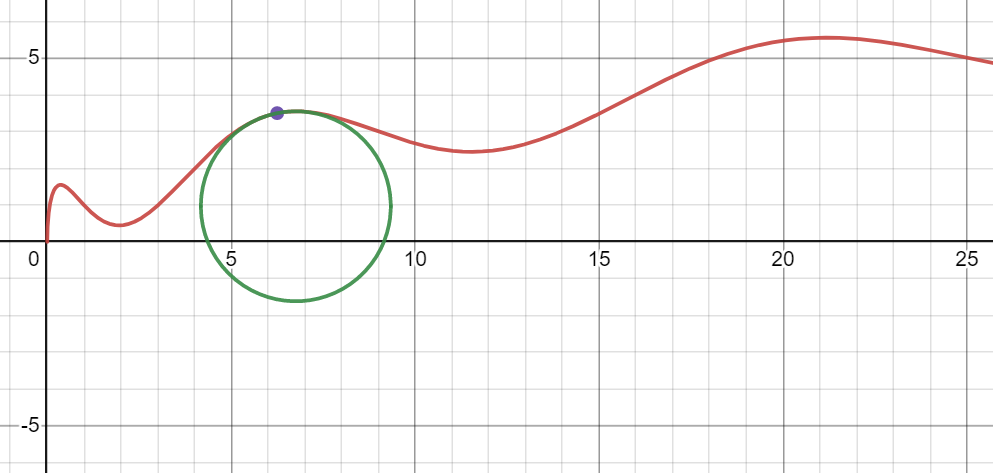
\includegraphics[scale=0.3]{Figures/osculatingcircles}
\end{center}
\end{example}

\begin{exercise}{Curvature and Evolutes}
Let $$\vcr(t)=\bmat{t\\ 2\sin(t)\\ 2\cos(t)}.$$
\vspace{1em}
\begin{enumerate}
\item Find $\vcT(t)$ and $\vcN(t)$, the tangent and normal vectors for $\vcr(t)$.
\vspace{1em}
\item Find $\kappa(t)$, the curvature of $\vcr(t)$.
\vspace{1em}
\item Find $\vcE(t)$, the evolute of $\vcr(t)$.
\end{enumerate}
\end{exercise}

\begin{exercise}{Curvature 2, Electric Boogaloo}
Let $$\vcr(t)=\bmat{t^2\\0\\t}.$$
\vspace{1em}
\begin{enumerate}
\item Find $\kappa(t)$, the curvature of $\vcr(t)$. (hint, it might be easier to calculate this using the second formula for curvature!)
\end{enumerate}
\end{exercise}